\begin{frame}
    \frametitle{Cámara Time of Flight}
    \note{https://en.wikipedia.org/wiki/Time-of-flight_camera}
    \scriptsize
    
    \begin{figure}[!h]
        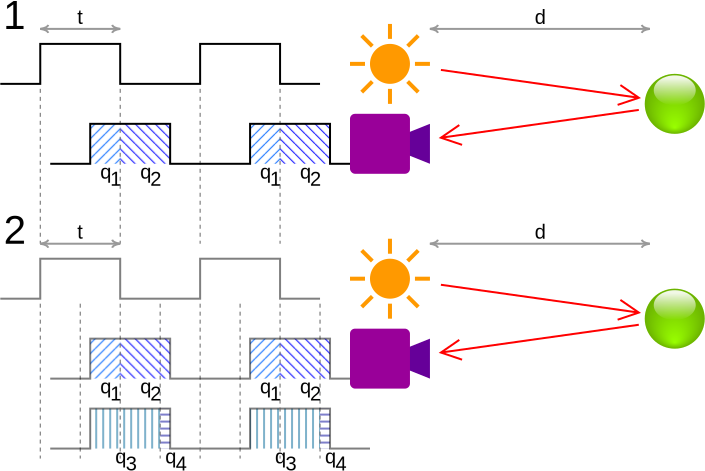
\includegraphics[width=0.4\columnwidth]{images/time_of_flight_camera.pdf}
    \end{figure}
    
    \begin{block}{Principio de funcionamiento}
        Funciona de manera similar a un lidar con la ventaja de que toda la escena 3D se captura al mismo tiempo y que no hay partes móviles. Este dispositivo utiliza una fuente de luz infrarroja modulada para determinar la distancia de cada píxel de un sensor Photonic Mixer Device (PMD).
    \end{block}
    
    \begin{itemize}
        \item Esteroceptivo
        \item Activo
        \item La precisión suele estimarse en un $\SI{1}{\percent}$ de la distancia medida, suelen tener un frame rate de unos $\SI{160}{\hertz}$
        \item La luz del entorno puede quemar la imagen (requiere píxeles con buen rango dinámico)
    \end{itemize}
    
\end{frame}